\documentclass[a4paper,10pt]{article} 
\usepackage[utf8]{inputenc}
\usepackage[a4paper]{geometry}
\usepackage[magyar]{babel}
\usepackage{amsmath}
\usepackage{amssymb}
\usepackage{pgf,tikz}
\usetikzlibrary{arrows}
\usepackage{caption}
\frenchspacing 
\pagestyle{empty}
\newcommand{\ki}[2]{\hfill {\it #1 (#2)}\medskip}
\newcommand{\vonal}{\hbox to \hsize{\hskip2truecm\hrulefill\hskip2truecm}}
\newcommand{\degre}{\ensuremath{^\circ}}
\newcommand{\tg}{\mathop{\mathrm{tg}}\nolimits}
\newcommand{\ctg}{\mathop{\mathrm{ctg}}\nolimits}
\newcommand{\arc}{\mathop{\mathrm{arc}}\nolimits}
\begin{document}
\begin{center} \Large {\em XX. Nemzetközi Magyar Matematika Verseny} \end{center}
\begin{center} \large{\em Bonyhád, 2011. március 11--15.} \end{center}
\smallskip
\begin{center} \large{\bf 10. osztály} \end{center}
\bigskip 

{\bf 1. feladat: }
Legyen egy háromszög három oldalának a hossza $a$, $b$ és $c$. Bizonyítsuk be, hogy
\[3 \le \frac{(a+b+c)^2}{ab+bc+ca} \le 4\]
Mikor állhat fenn egyenlőség?

\ki{Kántor Sándorné}{Debrecen}\medskip

{\bf Megoldás: } A feladatban szereplő kettős egyenlőtlenséget bontsuk két részre és végezzünk ekvivalens
átalakításokat.
\[3 \le \frac{(a+b+c)^2}{ab+bc+ca} \le 4\]
\[3(ab+bc+ca) \le (a+b+c)^2 \le 4(ab+bc+ca)\]

\textbf{a)} Bizonyítsuk először a bal oldalt:
\[3(ab+bc+ca) \le (a+b+c)^2, \eqno{(1)}\]
amiből a négyzetre emelést elvégezve és átrendezés után
\[a^2+b^2+c^2-ab-bc-ca\ge0.\]
Kettővel való beszorzás és a tagok csoportosítása után kapjuk, hogy
\[(a-b)^2+(b-c)^2+(c-a)^2\ge0,\]
ami minden valós $a$, $b$, $c$ értékre igaz, így az $(1)$ egyenlőtlenség is igaz.

Egyenlőség akkor és csak akkor áll fenn, ha $a=b=c$, tehát ha a háromszög szabályos.

\textbf{b)} Tekintsük most a jobb oldalt.
\[(a+b+c)^2 \le 4(ab+bc+ca) \eqno{(2)}\]
A négyzetre emelés és mindkét oldalból $2ab+2bc+2ca$ kivonás után
\[a2+b^2+c^2\le2(ab+bc+ca).\eqno{(2*)}\]
Mivel
\[2(ab+bc+ca)=a(b+c)+b(a+c)+c(a+b)\]
és a háromszög-egyenlőtlenségek szerint
\[a^2<a(b+c), \quad b^2<b(a+c), \quad c^2<c(a+b),\]
az egyenlőtlenségek összeadásával $(2*)$ igaz. Mivel $(2*)$-ot $(2)$-ből ekvivalens átalakításokkal kaptuk meg, így $(2)$ is igaz és egyenlőség soha nem áll fenn.

Mivel az átalakítások ekvivalensek, ezért a bizonyítást a visszafelé bizonyítás módszerére való hivatkozással lehet befejezni.

\medskip

\vonal
{\bf 2. feladat: } 
Oldjuk meg a következő egyenletrendszert a valós számok halmazán!
\begin{equation*}
\left.
\begin{aligned}
4x^2-3y&= xy^3 \\
x^2+x^3y^2&= 2y \\
\end{aligned}
\right\}
\end{equation*}

\ki{Balázsi Borbála}{Beregszász}\medskip

{\bf Megoldás: } Ha $x=0$ vagy $y=0$, az $(x;y)=(0;0)$ megoldást kapjuk.

Ha $x\ne0$ és $y\ne0$, az első egyenletet szorozzuk meg $x^2$-tel, a másodikat $y$-nal.
\begin{align*}
4x^4-3x^2y-x^3y^3&= 0 \\
x^2y+x^3y^3&= 2y^2 
\end{align*}
Adjuk össze $(1)$-et és $(2)$-t!
\[4x^4-2x^2y= 2y^2\]
Az első egyenletet nullára rendezés és 2-vel való osztás után szorzattá alakíthatjuk:
\[\left(y-x^2\right)\left(y+2x^2\right)= 0\]
Egy szorzat akkor és csak akkor nulla, ha legalább egy tényezője nulla, így két esetet különböz\-te\-tünk meg.

Ha $y=x^2$, akkor felhasználjuk az eredeti egyenletrendszer második egyenletét:
\begin{align*}
x^2+x^7&=2x^2\\
x^7&=x^2\\
x^5&=1
\end{align*}
Innen $x=1$, $y=1$.

Ha $y=-2x^2$, akkor is az eredeti egyenletrendszer második egyenletét használjuk:
\begin{align*}
x^2+4x^7&=-4x^2\\
4x^7&=-5x^2\\
x^5&=-\frac54\\
x&=-\sqrt[5]{\frac54}=-\sqrt[5]{\frac{40}{32}}=-\frac{\sqrt[5]{40}}{2}
\end{align*}
Visszahelyettesítve $y=-2x^2$-be
\[y=-2\left(-\frac{\sqrt[5]{40}}{2}\right)^2=-2\cdot\frac{\sqrt[5]{1600}}{4}=-\sqrt[5]{\frac{1600}{32}}=-\sqrt[5]{50}.\]

Tehát a megoldások:
\[(0;0), \quad (1;1), \quad \left(-\frac{\sqrt[5]{40}}{2};-\sqrt[5]{50}\right).\]

\medskip


\vonal
{\bf 3. feladat: } 
Az $AB$ szakaszon vegyük fel a $C$ és $D$ pontokat úgy, hogy $AC=CD=DB$ legyen és legyen $CDEF$ egy tetszőleges  paralelogramma. Legyen $G$ az $AE$ és $DF$, $H$ pedig a $BF$ és $CE$ metszéspontja. Bizonyítsuk be, hogy $AB=9GH$.

\ki{Olosz Ferenc}{Szatmárnémeti}\medskip

{\bf Megoldás: } 
Legyen $O$ a paralelogramma átlóinak metszéspontja, vegyük fel azokat a $K$ és $L$ pontokat, melyekre $K\in BF$ és $L\in AE$ és $DK\parallel CE$ és $CL\parallel DF$.

\begin{figure}[h!]
\begin{center}
{
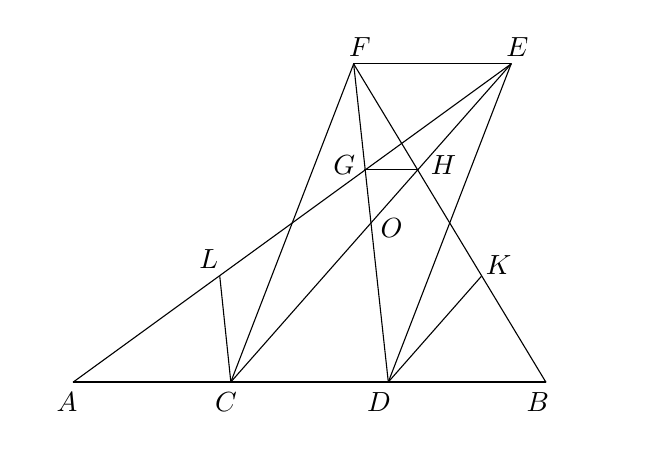
\begin{tikzpicture}[line cap=round,line join=round,>=triangle 45,x=2.0cm,y=2.0cm]
\clip(-0.29,-0.31) rectangle (3.49,2.25);
\draw (0,0)-- (3,0);
\draw (2,0)-- (2.78,2.02);
\draw (2.78,2.02)-- (1.78,2.02);
\draw (1.78,2.02)-- (1,0);
\draw (0,0)-- (2.78,2.02);
\draw (2,0)-- (1.78,2.02);
\draw (1,0)-- (2.78,2.02);
\draw (1.78,2.02)-- (3,0);
\draw (1.85,1.35)-- (2.19,1.35);
\draw (2.59,0.67)-- (2,0);
\draw (1,0)-- (0.93,0.67);
%\fill [color=black] (0,0) circle (1.5pt);
\draw[color=black] (-0.04,-0.13) node {$A$};
%\fill [color=black] (3,0) circle (1.5pt);
\draw[color=black] (2.95,-0.13) node {$B$};
%\fill [color=black] (1,0) circle (1.5pt);
\draw[color=black] (0.97,-0.13) node {$C$};
%\fill [color=black] (2,0) circle (1.5pt);
\draw[color=black] (1.94,-0.13) node {$D$};
%\fill [color=black] (2.78,2.02) circle (1.5pt);
\draw[color=black] (2.82,2.13) node {$E$};
%\fill [color=black] (1.78,2.02) circle (1.5pt);
\draw[color=black] (1.82,2.13) node {$F$};
%\fill [color=black] (1.85,1.35) circle (1.5pt);
\draw[color=black] (1.72,1.38) node {$G$};
%\fill [color=black] (2.19,1.35) circle (1.5pt);
\draw[color=black] (2.35,1.38) node {$H$};
%\fill [color=black] (1.89,1.01) circle (1.5pt);
\draw[color=black] (2.02,0.98) node {$O$};
%\fill [color=black] (2.59,0.67) circle (1.5pt);
\draw[color=black] (2.70,0.74) node {$K$};
%\fill [color=black] (0.93,0.67) circle (1.5pt);
\draw[color=black] (0.86,0.78) node {$L$};
\end{tikzpicture}
}
\end{center}
\caption*{A 3. feladathoz.}
\end{figure}

A paralelogramma átlói felezik egymást, ezért a $DFK$ háromszögben $OH$ középvonal és $DK=2\cdot OH$.

A $CBH$ háromszögben $DK$ középvonal és $CH=2\cdot DK=4\cdot OH$, ahonnan $CO=3\cdot OH$.

Hasonlóan bizonyítjuk, hogy $DO=3\cdot OG$.

A $COD$ és $HOG$ háromszögek hasonlók, ezért
\[\frac{CO}{OG}=\frac{DO}{GO}=\frac{CD}{HG}=3\].

Tehát $CD=3\cdot HG$ és $AB=3\cdot CD$, így $AB=9\cdot GH$.

\medskip


\vonal
{\bf 4. feladat: } 
Egy $2n$ oldalú, szimmetria-középponttal rendelkező konvex sokszöglap ($\mathcal{P}$) csúcspontjai közül kiválasztunk hármat, jelöljük őket $A$-val, $B$-vel és $C$-vel. Igazoljuk, hogy az $ABC$ háromszög $t$ területe nem nagyobb, mint  $\frac{T}{2}$, ahol $T$ a $\mathcal{P}$ sokszöglap területét jelöli.

\ki{Dálya Pál Péter}{Szeged}\medskip

{\bf Megoldás: } 
Jelölje $O$ a $\mathcal{P}$ szimmetria-középpontját és $A'$, $B'$, $C'$ rendre az $A$, $B$, $C$ pontok $O$-ra vonatkozó tükörképeit. Három esetet különböztetünk meg:

{\it I. eset.} Ha O illeszkedik az ABC háromszög egyik oldalára, akkor ez csakis az oldal felezőpontja lehet, hiszen ellenkező esetben a konvex sokszög kettőnél több csúcsa is illeszkedne az illető oldal egyenesre, ami konvex sokszög esetén kizárt. Ha a háromszög harmadik csúcsát tükrözzük a szemközti oldal felezőpontjára, $O$-ra, akkor egy paralelogrammát kapunk,  amelynek csúcsai a sokszög csúcsai közül valók, így a paralelogramma része a konvex sokszöglapnak, tehát $2t\le T$, vagyis $t\le \frac T 2$.

{\it II. eset.} Ha $O$ az $ABC$ háromszöglapon kívül van, akkor az $O$ ponton át húzhatunk egy olyan $e$ egyenest, amelyik nem metszi a háromszöglapot. Az $A$, $B$, $C$ pontok és az $A'$, $B'$, $C'$ tükörképek az $e$ egyenes különböző oldalán helyezkednek el. Tehát az $ABC$ és $A'B'C'$ egybevágó háromszöglapoknak nincs közös pontjuk és mindkettő a konvex sokszög része, így ebben az esetben is igaz, hogy $t \le \frac T 2$.

{\it III. eset.} Ha $O$ az $ABC$ háromszöglap belső pontja (lásd az \emph{ábrát}), akkor mivel az $A$, $B$, $C$, $A'$, $B'$, $C'$ pontok a konvex sokszög csúcsai, következik, hogy $AC'BA'CB'$ egy konvex hatszöglap, amely része a konvex sokszöglapnak. Nyilvánvalóan ahhoz, hogy a csúcsok tükörképei a háromszöglapon kívül kerüljenek, szükséges, hogy a szimmetria-középpont az $ABC$ háromszög középponti háromszögének belsejében legyen. 

\begin{figure}[h!]
\begin{center}
{
\definecolor{ffqqqq}{rgb}{1,0,0}
\definecolor{qqqqff}{rgb}{0,0,1}
\begin{tikzpicture}[line cap=round,line join=round,>=triangle 45,x=1.5cm,y=1.5cm]
\clip(-0.42,-1.02) rectangle (3.3,3.1);
\draw (0,0)-- (2.21,0);
\draw (2.21,0)-- (2,2.69);
\draw (2,2.69)-- (0,0);
\draw (2.88,1.96)-- (0.67,1.96);
\draw (0.67,1.96)-- (0.89,-0.73);
\draw (0.89,-0.73)-- (2.88,1.96);
\draw [color=qqqqff] (1,1.34)-- (1.11,0);
\draw [color=qqqqff] (1.11,0)-- (2.1,1.34);
\draw [color=qqqqff] (2.1,1.34)-- (1,1.34);
\draw [dotted] (2,2.69)-- (0.89,-0.73);
\draw [dotted] (2.21,0)-- (0.67,1.96);
\draw [dotted] (0,0)-- (2.88,1.96);
\draw [color=ffqqqq] (2.88,1.96)-- (2,2.69);
\draw [color=ffqqqq] (2,2.69)-- (0.67,1.96);
\draw [color=ffqqqq] (0.67,1.96)-- (0,0);
\draw [color=ffqqqq] (0,0)-- (0.89,-0.73);
\draw [color=ffqqqq] (0.89,-0.73)-- (2.21,0);
\draw [color=ffqqqq] (2.21,0)-- (2.88,1.96);
%\fill [color=black] (0,0) circle (1.5pt);
\draw[color=black] (-0.17,-0.01) node {$A$};
%\fill [color=black] (2.21,0) circle (1.5pt);
\draw[color=black] (2.35,0.01) node {$B$};
%\fill [color=black] (2,2.69) circle (1.5pt);
\draw[color=black] (2.06,2.82) node {$C$};
%\fill [color=black] (1.44,0.98) circle (1.5pt);
\draw[color=black] (1.24,1.03) node {$O$};
%\fill [color=black] (2.88,1.96) circle (1.5pt);
\draw[color=black] (3.01,2.09) node {$A'$};
%\fill [color=black] (0.67,1.96) circle (1.5pt);
\draw[color=black] (0.6,2.11) node {$B'$};
%\fill [color=black] (0.89,-0.73) circle (1.5pt);
\draw[color=black] (0.79,-0.87) node {$C'$};
\end{tikzpicture}
}
\end{center}
\caption*{A 4. feladathoz.}
\end{figure}

Jelölje $x$, $y$, $z$ az $O$ pontnak rendre a $BC$, $CA$, $AB$ egyenesektől mért távolságát; $a$, $b$, $c$ rendre a $BC$, $CA$, $AB$ oldalak hosszát; $m_a$, $m_b$, $m_c$ a megfelelő magasságokat, így mivel $t_{OBC} + t_{OCA} + t_{OAB} = t$, következik, hogy
\[\frac{ax}{2}+\frac{by}{2}+\frac{cz}{2}=t.\]
Könnyen belátható (a középpontos tükrözésből következik), hogy 
\[d(A',BC) = m_a-2x, \quad d(B',AC) = m_b-2y \quad \textrm{és} \quad d(C', AB) = m_c-2z.\]
Ezek alapján kiszámítható a konvex hatszöglap területe.
\begin{align*}
t_{AC'BA'CB'} &= t_{BA'C}+t_{CB'A}+t_{AC'B}+t \\
&= \frac{a\left(m_a-2x\right)}{2}+\frac{b\left(m_b-2y\right)}{2}+\frac{c\left(m_c-2z\right)}{2}+t \\
&= 4t-(ax+by+cz)=2t
\end{align*}
Mivel a konvex hatszöglap része az eredeti konvex sokszöglapnak, következik, hogy $2t\le T$, ami
igazolja a feladat állítását ebben az esetben is.

\medskip


\vonal
{\bf 5. feladat: } 
Hány olyan egyenlőszárú trapéz létezik, amelynek a kerülete 2011 és az oldalak mérőszáma egész szám?

\ki{Szabó Magda}{Szabadka}\medskip

{\bf Megoldás: } 
A trapéz oldalai legyenek ebben a sorrendben $a$, $c$, $b$, $c$; $a\ge b$ párhuzamos oldalak.

A trapéz kerülete 2011:
\begin{align*}
a+2c+b &= 2011\\
a+b&=2011-2c
\end{align*}
Tehát a párhuzamos oldalak összege páratlan szám, így nem lehetnek egyformák, amiből következik, hogy $a>b$.

Könnyű meggondolni, hogy igaz a következő is:
\[a<c+b+c,\]
azaz
\[2a<a+c+b+c=2011,\]
tehát $a\le1005$. Az $a$ valamely rögzített értékére $b$ az $\{1,2,3,...1005\}$ halmaz bármely $a$-nál kisebb eleme lehet, de paritásban különbözőnek kell lennie, hiszen az összegük páratlan szám. Tehát rögzített $a$-ra a lehetőségek száma $\left[\frac a 2\right]$.

Ha adott $a$ és $b$, akkor $c$ egyértelműen meghatározható (és ebből következően a trapéz is egyértelműen meghatározott), hiszen
\[c=\frac{2011-a-b}{2}\]

Ezekat felhasználva felírhatjuk az ilyen trapézok számát:
\begin{align*}
\sum_{a=1}^{1005} \left[\frac a 2\right]&=0+1+1+2+2+\ldots+501+501+502+502=\\
&= 2\cdot \sum_{i=1}^{502} i = 2\cdot\frac{502\cdot503}{2}=252506.
\end{align*}

\medskip


\vonal
{\bf 6. feladat: } 
Adott nyolc különböző pozitív egész szám a tízes számrendszerben. Képezzük bármely kettő (pozitív) különbségét, majd az így kapott 28 számot szorozzuk össze. 6-nak melyik az a legnagyobb kitevőjű hatványa, amivel ez a szorzat biztosan osztható?

\ki{Kiss Sándor}{Nyíregyháza}\medskip

{\bf Megoldás: } 
Egy szám akkor és csak akkor osztható 6-tal, ha osztható 2-vel és 3-mal.

Két szám különbsége csak akkor osztható 2-vel, ha azok paritása megegyezik (mindkettő páros vagy mindkettő páratlan.

Belátható, hogy négy páros és négy páratlan szám megadása esetén lesz a lehető legkevesebb páros tényező, ugyanis
\[\binom{x}{2}+\binom{8-x}{2}\ge2\binom{4}{2}\]

A négy párosból és a négy páratlanból is 6-6 darab 2-vel osztható tényezőt lehet képezni, a többi társítás páratlan lesz. Ez azt jelenti, hogy 2-nek a 12. hatványával biztosan osztható lesz
a 28 szám szorzata.

A hárommal való oszthatóság szempontjából a természetes számok algebrai alakja $3k$, $3k +1$ vagy $3k + 2$ lehet. Az azonos algebrai alakú számok különbsége osztható 3-mal.

Legkevesebb 3-mal osztható tényezőt akkor kapunk, ha a fenti alakú számok eloszlása 3, 3, 2, valamilyen sorrendben.

Ha valamelyik típusból 3 darab van, akkor abból 3 db hárommal osztható számot tudunk képezni. Ha valamelyikből csak 2, akkor 1 darab 3-mal oszthatót készíthetünk.

Így a 3 kitevője legalább 3 + 3 + 1 lesz, vagyis a 3 hetedik hatványával még biztosan osztható.

Összegezve: a 28 darab feladatbeli tényező a 6 hetedik hatványával még biztosan osztható. (A nyolcadikkal viszont nem feltétlenül, mert például az $\{1,2,3,\ldots 8\}$ esetén a szorzat csak 3-nak csak a 7. hatványával osztható.)
\end{document}